
\documentclass[
	12pt,				% tamanho da fonte
	openright,			% capítulos começam em pág ímpar (insere página vazia caso preciso)
	oneside,			% para impressão em recto e verso (twoside). Oposto a (oneside)
	a4paper,			% tamanho do papel. 
	chapter=TITLE,		% títulos de capítulos convertidos em letras maiúsculas
	section=TITLE,		% títulos de seções convertidos em letras maiúsculas
	sumario=abnt-6027-2012,
	english,			% idioma adicional para hifenização
	brazil,				% o último idioma é o principal do documento
	fleqn,				% equações alinhadas a esquerda (UDESC/CCT)+
	]{abntex2}

% ----------------------------------------------------------
% Pacotes básicos 
% ----------------------------------------------------------
\usepackage{amsmath}							% Pacote matemático
\usepackage{amssymb}							% Pacote matemático
\usepackage{amsfonts}							% Pacote matemático
%\usepackage{lmodern}							% Usa a fonte Latin Modern		
\usepackage{mathptmx} 							% Usa a fonte Times New Roman	 
\usepackage[T1]{fontenc}						% Selecao de codigos de fonte.
\usepackage[utf8]{inputenc}						% Codificacao do documento (conversão automática dos acentos)
% \usepackage{float}                              % Adiciona o pacote 
\usepackage{lastpage}							% Usado pela Ficha catalográfica
\usepackage{indentfirst}						% Indenta o primeiro parágrafo de cada seção.
\usepackage[dvipsnames,table]{xcolor}			% Controle das cores
\usepackage{graphicx}							% Inclusão de gráficos
\usepackage{microtype} 							% para melhorias de justificação
\usepackage{lipsum}								% para geração de dummy text
\usepackage[brazilian,hyperpageref]{backref}	% Paginas com as citações na bibl
\usepackage[alf,abnt-emphasize=bf,abnt-full-initials=yes]{abntex2cite}					% Citações padrão ABNT
%\usepackage[num]{abntex2cite}					% Citações padrão ABNT numérica
\usepackage{adjustbox}							% Pacote de ajuste de boxes
\usepackage{subcaption}							% Inclusão de Subfiguras e sublegendas		
\usepackage{enumitem}							% Personalização de listas
\usepackage{siunitx}							% Grandezas e unidades
\usepackage[section]{placeins}					% Manter as figuras delimitadas na respectiva seção com a opção [section]
\usepackage{multirow}							% Multi colunas nas tabelas
\usepackage{array,tabularx} 					% Pacotes de tabelas
\usepackage{booktabs} 							% Pacote de tabela profissonal
\usepackage{rotating}							% Rotacionar figuras e tabelas
\usepackage{xfrac}								% Fazer frações n/d em linha
\usepackage{bm}									% Negrito em modo matemático
\usepackage{xstring}							% Manipulação de strings
\usepackage{pgfplots}							% Pacote de Gráficos
\usepackage{tikz}								% Pacote de Figuras
\usepackage[american, cuteinductors,smartlabels, fulldiode, siunitx, americanvoltages, oldvoltagedirection, smartlabels]{circuitikz}						% Pacote de circuitos elétricos
\usepackage{chemformula}						% Pacote para fórmulas químicas
\usepackage{chngcntr}							% Pacte usado para deixar numeração de equações sequencial (UDESC/CCT)
\counterwithout{equation}{chapter}
% fonte: https://latex.org/forum/viewtopic.php?t=15392

% Comando para deixar numeração das equações contínua (1), (2), (3)... ao invés de organizar por capítulos (1.1)(1.2)... (2.1)(2.2)
%\renewcommand{\theequation}{\arabic{equation}}

%\numberwithin{equation}{section}

% Cabecalho cabeçalho somente com numeração de página 10pt
\makepagestyle{PagNumReduzida}
\makeevenhead{PagNumReduzida}{\ABNTEXfontereduzida\thepage}{}{}
\makeoddhead{PagNumReduzida}{}{}{\ABNTEXfontereduzida\thepage}
%fonte: https://github.com/abntex/abntex2/wiki/HowToCustomizarCabecalhoRodape
%fonte: Manual memoir seção 7.3 pg. 111 pdf http://linorg.usp.br/CTAN/macros/latex/contrib/memoir/memman.pdf 

% Personalização das opções das listas
\setlist[itemize]{leftmargin=\parindent}

% Citação online --- MODIFICAR ---
\newcommand{\citeshort}[1]{\citeauthoronline{#1}~(\citeyear{#1})}

\newcommand{\me}[1]{Elaborado pelo autor (#1).}

% Configuração do pgfplots
\pgfplotsset{compat=newest} %compat=1.14
\pgfplotsset{plot coordinates/math parser=false} 
\newlength\figureheight 
\newlength\figurewidth 

% Libraries do TiKz
\usetikzlibrary{quotes,angles,arrows}
\usetikzlibrary{through,calc,math}
\usetikzlibrary{graphs,backgrounds,fit}
\usetikzlibrary{shapes,positioning,patterns,shadows}
\usetikzlibrary{decorations.pathreplacing}
\usetikzlibrary{shapes.geometric}
\usetikzlibrary{arrows.meta}
\usetikzlibrary{external}

%\tikzexternalize[]
%\tikzexternalenable
%\tikzexternalize
%\tikzexternaldisable
%\tikzset{external/force remake}
%\tikzexternalize[shell escape=-enable-write18]

% Configurações do CircuiTiKz
\ctikzset{bipoles/thickness=1}
%\ctikzset{bipoles/length=1.2cm}
\ctikzset{monopoles/ground/width/.initial=.2}
\ctikzset{bipoles/resistor/height=0.25}
\ctikzset{bipoles/resistor/width=0.6}
\ctikzset{bipoles/capacitor/height=0.5}
\ctikzset{bipoles/capacitor/width=0.15}
\ctikzset{bipoles/generic/height=0.25}
\ctikzset{bipoles/generic/width=0.6}
%\ctikzset{bipoles/capacitor polar/length=0.5}
%\ctikzset{bipoles/diode/height=.375}
%\ctikzset{bipoles/diode/width=.3}
%\ctikzset{tripoles/thyristor/height=.8}
%\ctikzset{tripoles/thyristor/width=1}
\ctikzset{bipoles/vsourcesin/height=.5}
\ctikzset{bipoles/vsourcesin/width=.5}
\ctikzset{bipoles/cvsourceam/height=.6}
\ctikzset{bipoles/cvsourceam/width=.6}
%\ctikzset{tripoles/european controlled voltage source/width=.4}

\tikzstyle{every node}=[font=\footnotesize]
\tikzstyle{every path}=[line width=0.25pt,line cap=round,line join=round]
%\tikzstyle{every path}=[line cap=round,line join=round]


% Definição de cores MATLAB
\definecolor{matlab_blue}{rgb}	{         0,    0.4470,    0.7410}
\definecolor{matlab_orange}{rgb}{    0.8500,    0.3250,    0.0980}
\definecolor{matlab_yellow}{rgb}{    0.9290,    0.6940,    0.1250}
\definecolor{matlab_violet}{rgb}{    0.4940,    0.1840,    0.5560}
\definecolor{matlab_green}{rgb}	{	 0.4660,    0.6740,    0.1880}
\definecolor{matlab_lblue}{rgb}	{    0.3010,    0.7450,    0.9330}
\definecolor{matlab_red}{rgb}	{    0.6350,    0.0780,    0.1840}

% Personalização das legendas
\usepackage[format = plain, %hang
			justification = centering,
			labelsep = endash,
			singlelinecheck = false,
			skip = 6pt,
			listformat = simple]{caption}	

% Personalização das unidades
\sisetup{output-decimal-marker = {,}}
\sisetup{exponent-product = \cdot, output-product = \cdot}
\sisetup{tight-spacing=true}
\sisetup{group-digits = false}

% Personalizações de tipo de colunas de tabelas
\newcolumntype{L}[1]{>{\raggedright\let\newline\\\backslash\hspace{0pt}}m{#1}}
\newcolumntype{C}[1]{>{\centering\let\newline\\\arraybackslash\hspace{0pt}}m{#1}}
\newcolumntype{R}[1]{>{\raggedleft\let\newline\\\arraybackslash\hspace{0pt}}m{#1}}

% Personalizações de cores da UDESC
\definecolor{CapaAmareloUDESC}{RGB}{243,186,83}		% Especializacao
\definecolor{CapaVerdeUDESC}{RGB}{0,112,52}			% Mestrado
\definecolor{CapaVermelhoUDESC}{RGB}{171,35,21}		% Doutorado
\definecolor{CapaAzulUDESC}{RGB}{38,54,118} 		% Pós-Doutorado

% CONFIGURAÇÕES DE PACOTES
% Configurações do pacote backref
% Usado sem a opção hyperpageref de backref
\renewcommand{\backrefpagesname}{Citado na(s) página(s):~}
% Texto padrão antes do número das páginas
\renewcommand{\backref}{}
% Define os textos da citação
\renewcommand*{\backrefalt}[4]{
	\ifcase #1 %
	Nenhuma citação no texto.%
	\or
	Citado na página #2.%
	\else
	Citado #1 vezes nas páginas #2.%
	\fi}%

% alterando o aspecto da cor azul
%\definecolor{blue}{RGB}{41,5,195}

% informações do PDF
\makeatletter
\hypersetup{
	%pagebackref=true,
	pdftitle={\@title}, 
	pdfauthor={\@author},
	pdfsubject={\imprimirpreambulo},
	pdfcreator={LaTeX with abnTeX2},
	pdfkeywords={abnt}{latex}{abntex}{abntex2}{trabalho academico}, 
	colorlinks=true,       		% false: boxed links; true: colored links
	linkcolor=black,          	% color of internal links
	citecolor=black,        	% color of links to bibliography
	filecolor=black,      		% color of file links
	urlcolor=black,
	bookmarksdepth=4
}
\makeatother


\makeatletter
\newcommand{\includetikz}[1]{%
	\tikzsetnextfilename{#1}%
	\input{#1.tex}%
}
\makeatother

% ---
% Possibilita criação de Quadros e Lista de quadros.
% Ver https://github.com/abntex/abntex2/issues/176
%
\newcommand{\quadroname}{Quadro}
\newcommand{\listofquadrosname}{Lista de quadros}

\newfloat[chapter]{quadro}{loq}{\quadroname}
\newlistof{listofquadros}{loq}{\listofquadrosname}
\newlistentry{quadro}{loq}{0}

% configurações para atender às regras da ABNT
\setfloatadjustment{quadro}{\centering}
\counterwithout{quadro}{chapter}
\renewcommand{\cftquadroname}{\quadroname\space} 
\renewcommand*{\cftquadroaftersnum}{\hfill--\hfill}

\setfloatlocations{quadro}{hbtp} % Ver https://github.com/abntex/abntex2/issues/176
% ---


% Espaçamento depois do título
\setlength{\afterchapskip}{0.7\baselineskip}
% O tamanho do parágrafo é dado por:
\setlength{\parindent}{1.25cm}
% Controle do espaçamento entre um parágrafo e outro:
\setlength{\parskip}{0.0cm}  % tente também \onelineskip
%\SingleSpacing % Espaçamento simples 
\OnehalfSpacing % Espaçamento 1,5 (UDESC/CCT)
%\DoubleSpacing	% Espaçamento duplo

% ---
% Margens - NBR 14724/2011 - 5.1 Formato
% ---
\setlrmarginsandblock{3cm}{2cm}{*}
\setulmarginsandblock{3cm}{2cm}{*}
\checkandfixthelayout[fixed]
% ---


% To use externalize consider
%https://tex.stackexchange.com/questions/182783/tikzexternalize-not-compatible-with-miktex-2-9-abntex2-package
%Lauro Cesar digged into the problem until he came with a solution for me to test. And it Works!
%
%According to this link:
%
%The package calc changed the commands \setcounter and friends to be fragile. So you have to make them robust. The example below uses etoolbox with \robustify:
%
\usepackage{etoolbox}
\robustify\setcounter
\robustify\addtocounter
\robustify\setlength
\robustify\addtolength


%% How to silence memoir class warning against the use of caption package?
%% https://tex.stackexchange.com/questions/391993/how-to-silence-memoir-class-warning-against-the-use-of-caption-package
%\usepackage{silence}
%\WarningFilter*{memoir}{You are using the caption package with the memoir class}
%\WarningFilter*{Class memoir Warning}{You are using the caption package with the memoir class}

% --------------------------------------------------------
% INICIO DAS CUSTOMIZACOES PARA A UDESC
% --------------------------------------------------------

% --------------------------------------------------------
% Fontes padroes de part, chapter, section, subsection e subsubsection
% --------------------------------------------------------
% --- Chapter ---
\renewcommand{\ABNTEXchapterfont}{\fontseries{b}} %\bfseries
\renewcommand{\ABNTEXchapterfontsize}{\normalsize}
% --- Part ---
\renewcommand{\ABNTEXpartfont}{\ABNTEXchapterfont}
\renewcommand{\ABNTEXpartfontsize}{\LARGE}
% --- Section ---
\renewcommand{\ABNTEXsectionfont}{\normalfont}
\renewcommand{\ABNTEXsectionfontsize}{\normalsize}
% --- SubSection ---
\renewcommand{\ABNTEXsubsectionfont}{\fontseries{b}} %\bfseries
\renewcommand{\ABNTEXsubsectionfontsize}{\normalsize}
% --- SubSubSection ---
\renewcommand{\ABNTEXsubsubsectionfont}{\itshape}
\renewcommand{\ABNTEXsubsubsectionfontsize}{\normalsize}

\renewcommand{\ABNTEXsubsubsubsectionfont}{\normalfont}
\renewcommand{\ABNTEXsubsubsubsectionfontsize}{\normalsize}
% ---

% --------------------------------------------------------
% Fontes das entradas do sumario
% --------------------------------------------------------

\renewcommand{\cftpartfont}{\ABNTEXpartfont\selectfont}
\renewcommand{\cftpartpagefont}{\normalsize\selectfont}

\renewcommand{\cftchapterfont}{\ABNTEXchapterfont\selectfont}
\renewcommand{\cftchapterpagefont}{\normalsize\selectfont}

\renewcommand{\cftsectionfont}{\ABNTEXsectionfont\selectfont}
\renewcommand{\cftsectionpagefont}{\normalsize\selectfont}

\renewcommand{\cftsubsectionfont}{\ABNTEXsubsectionfont\selectfont}
\renewcommand{\cftsubsectionpagefont}{\normalsize\selectfont}

\renewcommand{\cftsubsubsectionfont}{\normalfont\itshape\selectfont}
\renewcommand{\cftsubsubsectionpagefont}{\normalsize\selectfont}

\renewcommand{\cftparagraphfont}{\normalfont\selectfont}
\renewcommand{\cftparagraphpagefont}{\normalsize\selectfont}

% --------------------------------------------------------
% Usando os pacotes hyperref, uppercase... 
% Para deixar a section do toc uppercase precisa de:
% --------------------------------------------------------
\usepackage{textcase}

\makeatletter

\let\oldcontentsline\contentsline
\def\contentsline#1#2{%
	\expandafter\ifx\csname l@#1\endcsname\l@section
	\expandafter\@firstoftwo
	\else
	\expandafter\@secondoftwo
	\fi
	{%
		\oldcontentsline{#1}{\MakeTextUppercase{#2}}%
	}{%
		\oldcontentsline{#1}{#2}%
	}%
}
\makeatother

% --------------------------------------------------------
% Renomenando as entradas de APÊNDICES E ANEXOS
% --------------------------------------------------------

\renewcommand{\apendicesname}{AP\^ENDICES}
\renewcommand{\anexosname}{ANEXOS}


% Manipulação de Strings
%\RequirePackage{xstring}

% Comando para inverter sobrenome e nome
\newcommand{\invertname}[1]{%
	\StrBehind{#1}{{}}, \StrBefore{#1}{{}}%
}%


% --------------------------------------------------------
% Alterando os estilos de Caption e Fonte
% --------------------------------------------------------
\makeatletter
% Define o comando \fonte que respeita as configurações de caption do memoir ou do caption
\renewcommand{\fonte}[2][\fontename]{%
	\M@gettitle{#2}%
	\memlegendinfo{#2}%
	\par
	\begingroup
	\@parboxrestore
	\if@minipage
	\@setminipage
	\fi
	\ABNTEXfontereduzida
	\configureseparator
	\captiondelim{\ABNTEXcaptionfontedelim}
	\@makecaption{#1}{\ignorespaces #2}\par
	\endgroup}


\captionstyle[\raggedright]{\raggedright}

\makeatother

\setlength{\cftbeforechapterskip}{0pt plus 0pt}
\renewcommand*{\insertchapterspace}{}

\newlength{\mylen}	% New length to use with spacing
\setlength{\mylen}{1pt}

\setlength{\cftbeforechapterskip}{\mylen}
\setlength{\cftbeforesectionskip}{\mylen}
\setlength{\cftbeforesubsectionskip}{\mylen}
\setlength{\cftbeforesubsubsectionskip}{\mylen}
\setlength{\cftbeforesubsubsubsectionskip}{\mylen}


% ---
% Ajuste das listas de abreviaturas e siglas ; e símbolos [Personalizada para UDESC com espaçamento 1,5]
% ---

% ---
% Redefinição da Lista de abreviaturas e siglas [Personalizada para UDESC com espaçamento 1,5]
\renewenvironment{siglas}{%
	\pretextualchapter{\listadesiglasname}
	\begin{symbols} 
		\setlength{\itemsep}{0pt}	% Ajuste para Espaçamento 1,5 (UDESC/CCT)
	}{% 
	\end{symbols}
	\cleardoublepage
}
% ---

% ---
% Redefinição da Lista de símbolos [Personalizada para UDESC com espaçamento 1,5]
\renewenvironment{simbolos}{%
	\pretextualchapter{\listadesimbolosname}
	\begin{symbols}
		\setlength{\itemsep}{0pt}	% Ajuste para Espaçamento 1,5 (UDESC/CCT)
	}{%
	\end{symbols}
	\cleardoublepage
}
% ---





% ---
% FIM DAS CUSTOMIZACOES PARA A  Universidade do Estado de Santa Catarina - UDESC/CCT
% ---





	% Incliu pacotes básicos 

% -----------------------------------------------------------------
% Você pode adicionar seus pacotes a partir desta linha;
% -----------------------------------------------------------------

%\usepackage[showframe,pass]{geometry}
%\usepackage[11,12]{pagesel}
\usepackage{float}
\usepackage{hyperref}


% -----------------------------------------------------------------
% Informações de dados para CAPA e FOLHA DE ROSTO
% -----------------------------------------------------------------

\titulo{Trabalho final de Econometria III - Replicação do artigo "Political systems, regime memory, and economic freedom"}%

\autor{Bruno Francisco {}Schaden}%

% ATENÇÃO: O símbolo {} indica o sobrenome para a ficha catalográfica.
% Exemplo: Sherlock Holmes {}da Silva para sobrenomes compostos;
% Exemplo: Arnold Alois {}Schwarzenegger para sobrenome simples.

\instituicao{Universidade do Estado de Santa Catarina, Centro de Ciências Tecnológicas, Programa de Pós--Graduação em Engenharia Elétrica}%

%\tipotrabalho{Tese (Doutorado)}
\tipotrabalho{Trabalho Acadêmico (Econometria III)}

%\preambulo{Tese apresentada ao Programa de Pós--Graduação em Engenharia Elétrica do Centro de Ciências Tecnológicas da Universidade do Estado de Santa Catarina, como requisito parcial para a obtenção do grau de Doutor em Engenharia Elétrica.}

\preambulo{Trabalho final de Econometria III, apresentado ao Curso de Ciências Econômicas da Universidade do Estado de Santa Catarina, como requisito parcial para a obtenção da nota da disciplina.}

\local{Florianópolis}%

\data{\the\year}%
% ---

% compila o indice
\makeindex

% -----------------------------------------------------------------
% Início do documento
% -----------------------------------------------------------------
\begin{document}

\selectlanguage{brazil}
\frenchspacing  % Retira espaço extra obsoleto entre as frases.

% -----------------------------------------------------------------
% ELEMENTOS PRÉ-TEXTUAIS
% -----------------------------------------------------------------
\pretextual

% Você pode comentar os elementos que não deseja em seu trabalho;

% A capa pode ser escolhida dentro do arquivo Capa.tex (TCC, Master, Doc, ...)
% ---
% Capa
% ---


% --------------------------------------------------------
% Capa Padrão
% --------------------------------------------------------
\renewcommand{\imprimircapa}{%
	\begin{capa}%
		\center

		{\fontseries{b}\selectfont\MakeTextUppercase{UNIVERSIDADE DO ESTADO DE SANTA CATARINA -- UDESC}}
		
		{\fontseries{b}\selectfont\MakeTextUppercase{CENTRO DE CIÊNCIAS DA ADMINISTRAÇÃO E SOCIOECONÔMICAS -- ESAG }}
		
		{\fontseries{b}\selectfont\MakeTextUppercase{GRADUAÇÃO -- CIÊNCIAS ECONÔMICAS}}
		
		\vfill
		
		{\fontseries{b}\selectfont\MakeTextUppercase{\normalsize\imprimirautor}}
		
		\vfill
		\begin{center}
			{\fontseries{b}\selectfont\MakeTextUppercase{\imprimirtitulo}}
		\end{center}
		\vfill
		
		\vfill
		
		{\fontseries{b}\selectfont\MakeTextUppercase{\imprimirlocal}}
		\par
		{\fontseries{b}\selectfont \imprimirdata}
		\vspace*{1cm}
	\end{capa}
}



\imprimircapa				% Capa padrão

					% Elemento Obrigatório
% ---
% Folha de rosto
% ---








% --------------------------------------------------------
% folha de rosto 
% --------------------------------------------------------

\makeatletter

\renewcommand{\folhaderostocontent}{
	\begin{center}
		
		{\fontseries{b}\selectfont\MakeTextUppercase{\imprimirautor}}
		
		\vfill
		
		\begin{center}
			{\fontseries{b}\selectfont\MakeTextUppercase{\imprimirtitulo}}
		\end{center}
	
		\vspace*{1.5cm}

		\abntex@ifnotempty{\imprimirpreambulo}{%
			\hspace{.45\textwidth}
			{\begin{minipage}{.5\textwidth}
					\SingleSpacing
					\imprimirpreambulo\par
					\vspace*{4pt}
					{\imprimirorientadorRotulo~\imprimirorientador\par}
					\abntex@ifnotempty{\imprimircoorientador}{%
						{\imprimircoorientadorRotulo~\imprimircoorientador}%
					}%
			\end{minipage}}%
		}%
	
		
		\vfill
		
	{\fontseries{b}\selectfont\MakeTextUppercase{\imprimirlocal}}
	\par
	{\fontseries{b}\selectfont \imprimirdata}
	\vspace*{1cm}
	\end{center}
}


% (o * indica que haverá a ficha bibliográfica)
% ---
\imprimirfolhaderosto
% ---


			% Elemento Obrigatório
% Caso não utilize a Ficha Catalográfica entre na folha de rosto e retire o * de dentro do arquivo FolhadeRosto
% 
% ---
% Inserir a ficha bibliografica
% ---

% Isto é um exemplo de Ficha Catalográfica, ou ``Dados internacionais de
% catalogação-na-publicação''. Você pode utilizar este modelo como referência. 
% Porém, provavelmente a biblioteca da sua universidade lhe fornecerá um PDF
% com a ficha catalográfica definitiva após a defesa do trabalho. Quando estiver
% com o documento, salve-o como PDF no diretório do seu projeto e substitua todo
% o conteúdo de implementação deste arquivo pelo comando abaixo:



% \begin{fichacatalografica}
%     \includepdf{fig_ficha_catalografica.pdf}
% \end{fichacatalografica}


%	\setlength{\parindent}{0cm}
%	\setlength{\parskip}{0pt}
\begin{fichacatalografica}
	%\sffamily
	%\rmfamily
	\ttfamily \hbadness=10000
	\vspace*{\fill}					% Posição vertical
	\begin{center}					% Minipage Centralizado
	Para gerar a ficha catalográfica de teses e \\ 
	dissertações acessar o link:  \\
	https://www.udesc.br/bu/manuais/ficha
	
	\vspace*{8pt}
	
%	\begin{minipage}[c]{8cm}
%	\centering \sffamily
%	 Ficha catalográfica elaborada pelo(a) autor(a), com auxílio do programa de geração automática da Biblioteca Setorial do CCT/UDESC
%	\end{minipage}
	\fbox{\begin{minipage}[c]{12.5cm}		% Largura
	\flushright
	{\begin{minipage}[c]{10.5cm}		% Largura
	\vspace{1.25cm}
	%\footnotesize
	\setlength{\parindent}{1.5em}
	\noindent \invertname{\imprimirautor} \par
	\imprimirtitulo{ }/{ }\imprimirautor. -- \imprimirlocal, \imprimirdata .\par
	\pageref{LastPage} p. : il. ; 30 cm.\par
	\vspace{1.5em}
	\imprimirorientadorRotulo~\imprimirorientador.\par
	\imprimircoorientadorRotulo~\imprimircoorientador.\par
	\imprimirtipotrabalho~--~\imprimirinstituicao, \imprimirlocal, \imprimirdata.\par
	\vspace{1.5em}
		1. Palavra-chave.
		2. Palavra-chave.
		3. Palavra-chave.
 		4. Palavra-chave.
		5. Palavra-chave.
		I. \invertname{\imprimirorientador}.
		II. \invertname{\imprimircoorientador}.
		III. \imprimirinstituicao.
		IV. Título. %
	\vspace{1.25cm}	%		
	\end{minipage}%
	}% 
	\end{minipage}}%
	
	\vspace*{0.5cm}
	
	\end{center}
\end{fichacatalografica}


%\begin{fichacatalografica}
%	\sffamily
%	\vspace*{\fill}					% Posição vertical
%	\begin{center}					% Minipage Centralizado
%	\fbox{\begin{minipage}[c][8cm]{13.5cm}		% Largura
%	\small
%	\imprimirautor
%	%Sobrenome, Nome do autor
%	
%	\hspace{0.5cm} \imprimirtitulo  / \imprimirautor. --
%	\imprimirlocal, \imprimirdata-
%	
%	\hspace{0.5cm} \pageref{LastPage} p. : il. (algumas color.) ; 30 cm.\\
%	
%	\hspace{0.5cm} \imprimirorientadorRotulo~\imprimirorientador\\
%	
%	\hspace{0.5cm}
%	\parbox[t]{\textwidth}{\imprimirtipotrabalho~--~\imprimirinstituicao,
%	\imprimirdata.}\\
%	
%	\hspace{0.5cm}
%		1. Palavra-chave1.
%		2. Palavra-chave2.
%		3. Palavra-chave3.
% 		4. Palavra-chave4.
%		5. Palavra-chave5.
%		I. Orientador.
%		II. Universidade xxx.
%		III. Faculdade de xxx.
%		IV. Título 			
%	\end{minipage}}
%	\end{center}
%\end{fichacatalografica}
% ---

	% Elemento Obrigatório (Verso da Folha)
% 
% ---
% Inserir errata
% ---
\begin{errata}
Elemento opcional. 

Exemplo:

\vspace{\onelineskip}

SOBRENOME, Prenome do Autor. Título de obra: subtítulo (se houver). Ano de depósito. Tipo do trabalho (grau e curso) - Vinculação acadêmica, local de apresentação/defesa, data.

\begin{table}[htb]
\center
\begin{tabular}{|p{2.4cm}|p{2cm}|p{3cm}|p{3cm}|}
  \hline
   \textbf{Folha} & \textbf{Linha}  & \textbf{Onde se lê}  & \textbf{Leia-se}  \\
    \hline
    1 & 10 & auto-conclavo & autoconclavo\\
   \hline
\end{tabular}
\end{table}

\end{errata}
% ---				% Elemento Opcional
% 
% ---
% Inserir folha de aprovação
% ---

% Isto é um exemplo de Folha de aprovação, elemento obrigatório da NBR
% 14724/2011 (seção 4.2.1.3). Você pode utilizar este modelo até a aprovação
% do trabalho. Após isso, substitua todo o conteúdo deste arquivo por uma
% imagem da página assinada pela banca com o comando abaixo:
%
% \includepdf{folhadeaprovacao_final.pdf}
%
\begin{folhadeaprovacao}



	\begin{center}
		{\fontseries{b}\selectfont\MakeTextUppercase{\normalsize\imprimirautor}}
	\end{center}
    \vfill
    
	\vfill
	\begin{center}
		{\fontseries{b}\selectfont\MakeTextUppercase{\imprimirtitulo}}
	\end{center}
	\vfill

    
\abntex@ifnotempty{\imprimirpreambulo}{%
	\hspace{.45\textwidth}
	{\begin{minipage}{.5\textwidth}
			\SingleSpacing
			\imprimirpreambulo\par
			\vspace*{4pt}
			{\imprimirorientadorRotulo~\imprimirorientador\par}
			\abntex@ifnotempty{\imprimircoorientador}{%
				{\imprimircoorientadorRotulo~\imprimircoorientador}%
			}%
	\end{minipage}}%
}%


\vfill
        
	 \begin{center}
	 	
    	{\fontseries{b}\selectfont BANCA EXAMINADORA: }
    	\vspace*{1.75cm}
    
		Nome do Orientador e Titulação \par
		Nome da Instituição
	 \end{center}
	
    {Membros:} 
    
	\begin{center}
		\vspace*{1.25cm}
		Nome do Orientador e Titulação \par
		Nome da Instituição
		
		\vspace*{1.25cm}
		Nome do Orientador e Titulação \par
		Nome da Instituição
		
		\vspace*{1.25cm}
		Nome do Orientador e Titulação \par
		Nome da Instituição

	
	\end{center}
    
    \vspace*{\fill}  
    \begin{center}
    {\imprimirlocal, 01 de maio de \imprimirdata}
	\end{center}
    \vspace*{0.25cm}  
\end{folhadeaprovacao}
% ---




%\textbf{	{Orientador: \vspace{-16pt} }
%	\assinatura{\textbf{Prof. \imprimirorientador , Dr.} \\ Univ. XXX} 
%	{Coorientador: \vspace{-16pt}}   
%	\assinatura{\textbf{Prof. \imprimircoorientador , Dr.} \\ Univ. XXX}
%	
%	{Membros: \vspace{-16pt} } 
%	
%	% --- Exemplo de assinaturas em sequência ---       
%	\setlength{\ABNTEXsignwidth}{8.5cm}
%	
%	\assinatura{\textbf{Prof. Professor, Dr.} \\ Univ. XXX}
%	\assinatura{\textbf{Prof. Professor, Dr.} \\ Univ. XXX}
%	\assinatura{\textbf{Prof. Professor, Dr.} \\ Univ. XXX}
%	
%	% --- Exemplo de assinaturas lado a lado ---
%	\setlength{\ABNTEXsignwidth}{7.5cm}
	%
	%    \noindent\hfill\assinatura*{\textbf{Prof. Professor, Dr.} \\ Univ. XXX}%
	%    \hfill%
	%    \assinatura*{\textbf{Prof. Professor, Dr.} \\ Univ. XXX}%
	%    \hfill
	%    
	%    \noindent\hfill\assinatura*{\textbf{Prof. Professor, Dr.} \\ Univ. XXX}%
	%    \hfill%
	%    \assinatura*{\textbf{Prof. Professor, Dr.} \\ Univ. XXX}%
	%    \hfill}		% Elemento Obrigatório
% ---
% Dedicatória
% ---
\begin{dedicatoria}
   \vspace*{\fill}
%   \begin{flushright}
%   \noindent
%	Este trabalho é dedicado às crianças adultas que,\\
%	quando pequenas, sonharam em se tornar cientistas. 
%   \end{flushright}

{%
	\noindent\hspace{.5\textwidth}
	{\begin{minipage}{.5\textwidth}
			\begin{flushleft}
				Dedico este trabalho ao Professor Rafael Bressan, cuja habilidade em ensinar Econometria III transformou cada aula em uma verdadeira aventura. Entre momentos de desespero e epifanias matemáticas, obrigado por me ajudar a descobrir que, apesar de todas as adversidades, eu sou mais forte do que imaginava. Afinal, como dizia Muhammad Ali, "Sofra agora e viva o resto da sua vida como um campeão". E, claro, por me mostrar que a econometria, assim como a vida, pode ser vencida com um pouco de coragem e muita persistência.
			\end{flushleft}
	\end{minipage}}%
\vspace*{3cm}
}%

\end{dedicatoria}
% ---
			% Elemento Opcional
% ---
% Agradecimentos
% ---
\begin{agradecimentos}
    Gostaria de expressar minha mais sincera gratidão a todos que me apoiaram ao longo deste semestre, especialmente durante os intermináveis desafios de Econometria III. Quem diria que, em meio a tantos gráficos, fórmulas complexas e noites insones, eu conseguiria sobreviver? A cada aula, eu perdia um pouco mais da minha esperança de entender aquele universo, mas, de alguma forma milagrosa, consegui chegar ao fim.

    Agradeço aos meus remanescentes colegas de classe, que compartilharam comigo o desespero e a luta para decifrar aqueles enigmas econométricos. À minha família e amigos, por me suportarem nos momentos em que eu dizia que nunca conseguiria entender essa disciplina. E, claro, ao café, meu fiel companheiro nas madrugadas de estudo.
    
    Enfim, dedico este trabalho a todos que acreditaram que eu poderia superar Econometria III, mesmo quando eu mesmo duvidava disso. Aos futuros estudantes dessa disciplina, desejo força, pois se eu consegui, talvez qualquer um consegue!

\end{agradecimentos}
% ---		% Elemento Opcional
% ---
% Epígrafe
% ---
\begin{epigrafe}
    \vspace*{\fill}
%	\begin{flushright}
%		\textit{``Eu não falhei, encontrei 10 mil soluções que não davam certo.'' (EDISON, [19--])}
%	\end{flushright}
{%
	\noindent\hspace{.5\textwidth}
	{\begin{minipage}{.5\textwidth}
		\begin{flushright}
			``Liberdade significa responsabilidade. É por isso que tanta gente tem medo dela.'' (GEORGE BERNARD SHAW, [18--])
		\end{flushright}
	\end{minipage}}%
	\vspace*{3cm}
}%
\end{epigrafe}
% ---				% Elemento Opcional
% ---
% RESUMOS
% ---

% resumo em português
\setlength{\absparsep}{18pt} % ajusta o espaçamento dos parágrafos do resumo
\begin{resumo}
    O artigo "Sistemas políticos, memória de regime e liberdade econômica" de Peter Calcagno, Beatriz Maldonado, Todd Nesbit e Mary Frances Zeager investiga a influência da memória de regimes passados na liberdade econômica de um país. Os autores desenvolvem uma medida inovadora de memória de regime e analisam o efeito geracional de regimes anteriores na liberdade econômica. Por meio de um estudo com 144 países entre 1970 e 2015, o artigo destaca que a memória de regime pode promover melhorias na liberdade econômica em nações historicamente democráticas, enquanto desencoraja em países com histórico autocrático. Esses resultados contribuem para a compreensão de como a cultura, as tradições e as instituições passadas impactam as políticas econômicas atuais.

 \textbf{Palavras-chave}: Sistemas políticos. Memória de regime. Liberdade Econômica. Cultura. Instituições.
\end{resumo}
				% Elemento Obrigatório
% % ---
% Abstract
% ---

% resumo em inglês
\begin{resumo}[Abstract]
 \begin{otherlanguage*}{english}
   Elemento obrigatório para todos os trabalhos de conclusão de curso. Opcional para os demais trabalhos acadêmicos, inclusive para artigo científico. Constitui a versão do resumo em português para um idioma de divulgação internacional. Deve aparecer em página distinta e seguindo a mesma formatação do resumo em português.

   \textbf{Keywords}: Keyword 1. Keyword 2. Keyword 3. Keyword 4. Keyword 5.
 \end{otherlanguage*}
\end{resumo}
				% Elemento Obrigatório

% ---
% inserir lista de ilustrações
% ---
\pdfbookmark[0]{\listfigurename}{lof}
\listoffigures*
\cleardoublepage
% ---

% ---
% inserir lista de quadros
% ---
%\pdfbookmark[0]{\listofquadrosname}{loq}
%\listofquadros*
%\cleardoublepage
% ---


% ---
% inserir lista de tabelas
% ---
\pdfbookmark[0]{\listtablename}{lot}
\listoftables*
\cleardoublepage
% ---

% ---
% inserir lista de abreviaturas e siglas
% ---
\begin{siglas}
	\item[ABNT] Associação Brasileira de Normas Técnicas
	\item[BU] Biblioteca Universitária
	\item[IN] Instrução Normativa
	\item[NBR] Normas Técnicas Brasileiras
	\item[TCC] Trabalho de Conclusão de Curso
	\item[Udesc] Universidade do Estado de Santa Catarina
\end{siglas}
% ---

% ---
% inserir lista de símbolos
% ---


\begin{simbolos}
  \item[@] Arroba
  \item[\%] Porcento
  \item[$^\circ$C] Graus Celsius
  \item[Ca] Cálcio
\end{simbolos}

% ---
				% Elemento Opcional
% ---
% inserir o sumario
% ---
\pdfbookmark[0]{\contentsname}{toc}
\tableofcontents*
\cleardoublepage
% ---
				% Elemento Obrigatório

% -----------------------------------------------------------------
% ELEMENTOS TEXTUAIS
% -----------------------------------------------------------------
\textual

\pagestyle{PagNumReduzida}						% Comando para cabeçalho somente com numeração de página 10pt
\aliaspagestyle{chapter}{PagNumReduzida}		% Deixar numeração da primeira página com tamanho igual ao resto da numeração
% ref.: https://groups.google.com/g/abntex2/c/CP7g8ZMgi-c/m/KjfEnn5b9a4J


% ---- Mantenha está estrutura, assim você deixa o trabalho mais organizado -------


%\chapter{Introdução}


\chapter{Do Artigo Científico de Replicação}

O estudo de Calcagno et al. (2024) explora como sistemas políticos e a memória de regimes anteriores influenciam a liberdade econômica atual. A liberdade econômica é um conceito crítico que afeta o desenvolvimento econômico e social dos países. Este trabalho objetiva replicar os métodos e resultados de Calcagno et al. (2024) para confirmar a robustez das suas conclusões.

A motivação para esta replicação reside na importância de verificar a reprodutibilidade das pesquisas acadêmicas. Estudos replicados com sucesso reforçam a validade das teorias propostas e aumentam a confiança na literatura científica existente. A abordagem metodológica e os dados utilizados são detalhados nas seções subsequentes.


\section{Fonte dos Dados}
Os dados utilizados nesta replicação são provenientes das mesmas fontes mencionadas por Calcagno et al. (2024). Utilizamos o dataset replicação composto de liberdade econômica do Fraser Institute (2022) e variáveis políticas do Polity IV Project. Estes conjuntos de dados fornecem uma cobertura ampla e detalhada de indicadores econômicos e políticos ao longo do tempo.

Adicionalmente, também é incorporado no dataset dados demográficos e econômicos do Banco Mundial para controlar variáveis que possam influenciar a liberdade econômica. Estes dados permitem uma análise comparativa robusta entre diferentes países e regimes ao longo das últimas décadas.

\section{Memória de Regime}
A metodologia replicada segue os passos descritos por Calcagno et al. (2024) somente mudando o softwere de análise de Stata para Python. Utilizamos modelos de regressão linear múltipla para analisar a relação entre sistemas políticos, memória de regime e liberdade econômica. A variável dependente é o índice de liberdade econômica, enquanto as variáveis independentes incluem indicadores políticos e demográficos.

Para capturar os efeitos das mudanças institucionais lentas associadas à mudança de regime, utilizamos duas variáveis para construir nossa medida de memória de regime. Durable é uma variável de contagem que registra o tempo desde a mudança de regime mais recente. Para registrar um efeito na memória de regime, a pontuação máxima de durable para um determinado regime deve ser maior que zero. Polity2 controla o tipo de regime e varia de -10 a 10, com uma pontuação mais baixa indicando um regime mais autocrático e uma pontuação maior indicando um regime mais democrático.

Nossa medida de memória de regime de um país é melhor descrita como uma média ponderada das pontuações de polity2 pelo regime em que os pesos são determinados pela pontuação de durable de cada regime. A construção ampla é descrita da seguinte forma:

\[
\text{RegimeMemory}_{it} = \frac{\sum_{r=0}^{R} \left( w_{(t-1)r} \cdot \text{Polity2}_{(t-1-k)r} \right)}{\sum_{r=0}^{R} w_{(t-1)r}}
\]

onde $i$ e $t$ são índices para país e ano, respectivamente, e $r$ é o índice para o regime. Todas as referências temporais no lado direito são defasadas de modo que a memória de regime não é influenciada diretamente pelas pontuações contemporâneas de polity e durable — ela é destinada a representar puramente a memória dos regimes passados. O subscrito $k$ indexa o número de anos desde o término do regime anterior. Os pesos dos regimes são atribuídos com um valor inicial de um no primeiro ano de existência do regime. A influência desse regime, e portanto seu peso, é assumida como crescente a uma taxa de desconto constante (2,5\% e 12,5\% para os resultados principais apresentados aqui) a cada ano adicional em que o regime está em vigor. Uma vez que um regime termina, o peso atribuído à contribuição desse regime para a memória de regime começa a diminuir na mesma taxa de desconto. Nosso período de amostra para nossa análise de regressão começa em 1970; no entanto, a medida de memória de regime para um determinado país inclui a influência descontada de todos os regimes passados incluídos no conjunto de dados Polity IV.

\begin{figure}[h!]
    \centering
    \caption{Variável de memória de regime para Chile e França entre 1970 e 2015, utilizando taxas de desconto de 2,5\% e 12,5\%, assim como a medida de cálculo alternativa.}
    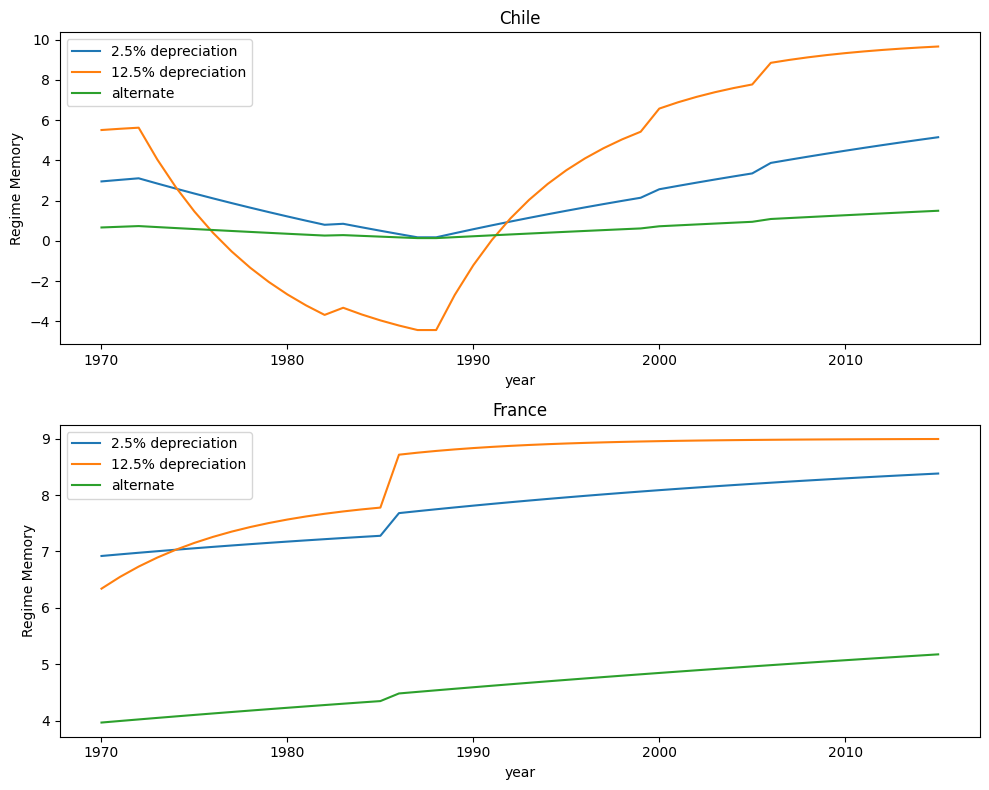
\includegraphics[width=0.8\textwidth]{Textuais/chile.png}
    \fonte{Replicação - Elaborado pelos autores.}
\end{figure}

\section{Metodologia Empírica}

A análise de regressão realizada utiliza o modelo de efeitos fixos para examinar a relação entre memória de regime e liberdade econômica. Este modelo permite controlar variáveis não observadas que são constantes ao longo do tempo, mas variam entre os países. A especificação do modelo é dada pela seguinte equação:

\begin{equation}
    \text{EFW}_{it} = \beta_1 \text{RegimeMemory}_{it} + \mathbf{X}_{it-1} \boldsymbol{\delta} + \Phi_t + \epsilon_{it} \quad 
\end{equation}

onde $i$ representa o índice de país e $t$ representa o índice de ano. Para explicar como a memória de regime afeta a liberdade econômica de um país, utilizamos o índice de Liberdade Econômica do Mundo (EFW) do projeto Economic Freedom of the World como nossa medida de liberdade econômica (Gwartney et al., 2022). O índice varia de 0 a 10, com pontuações mais baixas denotando menos liberdade econômica e pontuações mais altas denotando mais liberdade.


\chapter{Resultados}

\section{Descrição dos Dados}
As estatísticas descritivas das variáveis foram reproduzidas quase perfeitamente, como mostrado na Tabela \ref{tab:tabela_descritiva}. A diferença encontrada nos números é de orderm de $10^{-2}$, o que é aceitável dada a natureza dos cálculos. 

\begin{table}[htbp]
    \centering
    \renewcommand{\arraystretch}{1.1}
    \captionsetup{font=small}
    \caption{Estatísticas Descritivas.}
    \label{tab:tabela_descritiva}
    \scriptsize % Ajusta a fonte para tamanho 10
    \begin{tabular}{lrrrrrrrr}
        \toprule
        \textbf{Variável} & \textbf{N} & \textbf{Média} & \textbf{Desv. Padrão} & \textbf{Mín.} & \textbf{25\%} & \textbf{50\%} & \textbf{75\%} & \textbf{Máx.} \\
        \midrule
        EFW index interpolated & 4697 & 6.14 & 1.30 & 2.37 & 5.18 & 6.20 & 7.18 & 8.85 \\
        EFW index not interpolated & 2534 & 6.53 & 1.16 & 2.37 & 5.75 & 6.65 & 7.44 & 8.85 \\
        2.5\% discount & 4697 & 0.38 & 6.05 & -10.0 & -4.93 & -0.54 & 6.00 & 10.0 \\
        5\% discount & 4697 & 1.01 & 6.34 & -10.0 & -4.84 & 0.79 & 7.00 & 10.0 \\
        7.5\% discount & 4697 & 1.43 & 6.51 & -10.0 & -4.72 & 2.01 & 7.90 & 10.0 \\
        10\% discount & 4697 & 1.73 & 6.64 & -10.0 & -4.65 & 3.03 & 8.03 & 10.0 \\
        12.5\% discount & 4697 & 1.95 & 6.73 & -10.0 & -4.59 & 3.70 & 8.61 & 10.0 \\
        15\% discount & 4697 & 2.10 & 6.79 & -10.0 & -4.63 & 4.00 & 8.89 & 10.0 \\
        Alternative & 4697 & 0.27 & 6.20 & -10.0 & -4.93 & 0.69 & 4.30 & 10.0 \\
        Net ODA as \% of GDP & 4697 & 3.28 & 5.59 & -0.40 & 0.00 & 0.69 & 3.07 & 81.43 \\
        Resource rent as \% of GDP & 4697 & 7.05 & 9.75 & 0.00 & 0.00 & 3.07 & 9.21 & 79.74 \\
        Real GDP per capita & 4697 & 11224.56 & 16503.12 & 157.10 & 1262.87 & 3731.68 & 14263.96 & 114047.91 \\
        GDP growth & 4697 & 3.67 & 4.94 & -50.25 & -4.93 & 0.79 & 7.00 & 39.49 \\
        War Dummy & 4697 & 0.09 & 0.28 & 0 & 0 & 0 & 0 & 1 \\
        Christian Dummy & 4697 & 0.63 & 0.48 & 0 & 0 & 1 & 1 & 1 \\
        UK legal origin & 4697 & 0.30 & 0.46 & 0 & 0 & 0 & 1 & 1 \\
        French legal origin & 4697 & 0.56 & 0.50 & 0 & 0 & 1 & 1 & 1 \\
        Coup d'etats & 4477 & 0.04 & 0.21 & 0 & 0 & 0 & 0 & 1 \\
        Gini & 3530 & 39.07 & 8.84 & 20.30 & 32.40 & 39.60 & 45.07 & 65.40 \\
        \bottomrule
    \end{tabular}
    \fonte{Elaborado pelos autores.}
\end{table}


\section{SEÇÃO SECUNDÁRIA}

A ABNT indica a elaboração de uma lista de ilustrações com todos os itens arrolados e designados por seu nome específico, conforme a ordem que aparecem no texto (Figura 1, Fotografia 1, Gráfico 1, Quadro 1, entre outros). Também recomenda, quando necessário, a elaboração de lista própria para cada tipo de ilustração. No entanto, não determina um número mínimo de ilustrações para tal lista específica.

\begin{table}
	\caption{Tabela 3 do Artigo Original.}
	\label{tab:tabela3}
	\resizebox{\textwidth}{!}{\begin{tabular}{lcccc}
	\toprule
	Dependent variable & EFW index-interpolate (2.50\%) & EFW index-interpolate (12.50\%) & EFW index (2.50\%) & EFW index (12.50\%) \\
	\midrule
	Regime memory & 0.043 & 0.045 & 0.024 & 0.037 \\
	Net ODA as \% of GDP & 0.020 & 0.020 & 0.021 & 0.021 \\
	Resource rent as \% of GDP & -0.023 & -0.021 & -0.028 & -0.024 \\
	ln(GDP per capita) & 0.492 & 0.499 & 0.476 & 0.468 \\
	GDP Growth & 0.019 & 0.019 & 0.021 & 0.020 \\
	War Dummy & -0.234 & -0.209 & -0.195 & -0.200 \\
	Christian Dummy & -0.143 & -0.185 & 0.029 & -0.051 \\
	British legal origin & 0.089 & 0.162 & 0.125 & 0.177 \\
	French legal origin & -0.065 & -0.047 & -0.040 & -0.019 \\
	Number of observations & 4697 & 4697 & 2534 & 2534 \\
	R2 & 0.732 & 0.738 & 0.730 & 0.742 \\
	\bottomrule
	\end{tabular}}
	\end{table}


	\begin{table}
		\caption{Tabela 4 do Artigo Original.}
		\label{tab:tabela4}
		\resizebox{\textwidth}{!}{\begin{tabular}{lcccc}
		\toprule
		Dependent variable & EFW index-interpolate (2.50\%) & EFW index-interpolate (12.50\%) & EFW index (2.50\%) & EFW index (12.50\%) \\
		\midrule
		Regime memory & 0.045 & 0.046 & 0.045 & 0.050 \\
		Net ODA as \% of GDP & 0.021 & 0.021 & 0.021 & 0.022 \\
		Resource rent as \% of GDP & -0.023 & -0.021 & -0.026 & -0.023 \\
		ln(GDP per capita) & 0.485 & 0.493 & 0.464 & 0.481 \\
		GDP Growth & 0.020 & 0.019 & 0.032 & 0.032 \\
		War Dummy & -0.244 & -0.222 & -0.193 & -0.167 \\
		Christian Dummy & -0.132 & -0.178 & -0.049 & -0.113 \\
		British legal origin & 0.077 & 0.156 & 0.061 & 0.148 \\
		French legal origin & -0.072 & -0.050 & -0.143 & -0.120 \\
		Coup Dummy & -0.039 & -0.021 & -0.131 & -0.102 \\
		Gini Disposable & NA & NA & 0.002 & 0.004 \\
		Number of observations & 4477 & 4477 & 3462 & 3462 \\
		R2 & 0.727 & 0.733 & 0.714 & 0.724 \\
		\bottomrule
		\end{tabular}}
		\end{table}
Nesse caso, a BU Udesc estabelece a elaboração de listas específicas para cada tipo de ilustração somente quando existirem muitos itens de cada tipo: cinco (5) ou mais (mais do que cinco desenhos, gráficos etc.). Caso contrário, elabora-se uma única lista, denominada “Lista de ilustrações” com os elementos ordenados conforme aparecem no texto, nominando-os “Figura” e, portanto, não diferenciando fotografia, gráfico, quadro e outros.


\subsection{Seção terciária}

O vídeo fornece uma maneira poderosa de ajudá-lo a provar seu argumento. Ao clicar em Vídeo Online, você pode colar o código de inserção do vídeo que deseja adicionar.

\subsubsection{Seção quaternária}

O vídeo fornece uma maneira poderosa de ajudá-lo a provar seu argumento. Ao clicar em Vídeo Online, você pode colar o código de inserção do vídeo que deseja adicionar. Você também pode digitar uma palavra-chave para pesquisar online o vídeo mais adequado ao seu documento. 


\begin{figure}
	\centering
	\caption{Exemplo de paginação.}
	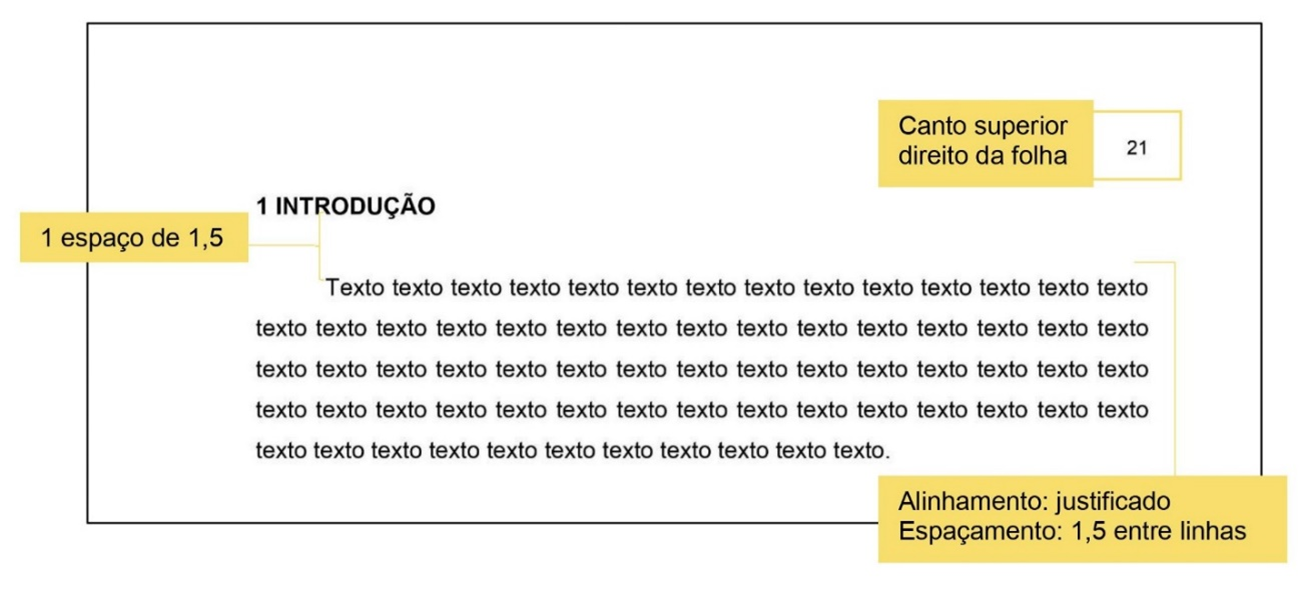
\includegraphics[scale=1]{Textuais/Picture1.png}
	\fonte{Elaborada pelos autores (2020), com base na NBR 14724 (2011).}
\end{figure}


\subsubsubsection{Seção quinaria}



O vídeo fornece uma maneira poderosa de ajudá-lo a provar seu argumento. Ao clicar em Vídeo Online, você pode colar o código de inserção do vídeo que deseja adicionar. Você também pode digitar uma palavra-chave para pesquisar online o vídeo mais adequado ao seu documento. Para dar ao documento uma aparência profissional, o Word\footnote{O Microsoft Word é um processador de texto produzido pela Microsoft Office foi criado por Richard Brodie para computadores IBM PC com o sistema operacional DOS em 1983.} fornece designs de cabeçalho, rodapé, folha de rosto e caixa de texto que se complementam entre si. Por exemplo, você pode adicionar uma folha de rosto, um cabeçalho e uma barra lateral correspondentes.

\begin{table}[!htbp]
	\centering
	%	\small
	\renewcommand{\arraystretch}{1.1}
	\caption{Modelo de tabela.}%
	\label{tab:tabela_exemplo}
	\begin{tabular}{ L{4cm}  R{3cm} || L{4cm}  R{3cm}  }
		\hline
		Município		& População Estimada & Município		& População Estimada 		\\ 
		\hline
		Abdon Batista		& 2630	& Bom Jesus				& 2821 \\ 
		Abelardo Luz		& 17717	& Bom Jesus do Oeste	& 2156 \\ 
		Agrolândia			& 10272	& Bom Retiro			& 9598 \\ 
		Agronômica			& 5306	& Bombinhas				& 17477 \\ 
		Água Doce			& 7132	& Botuverá				& 4943 \\ 
		Águas de Chapecó	& 6379	& Braço do Norte		& 31765 \\ 
		\hline
	\end{tabular}
	\vspace{2mm}
	\fonte{Adaptado de IBGE (2015).}
\end{table}

Clique em Inserir e escolha os elementos desejados nas diferentes galerias.

\begin{figure}
	\centering
	\caption{População.}
	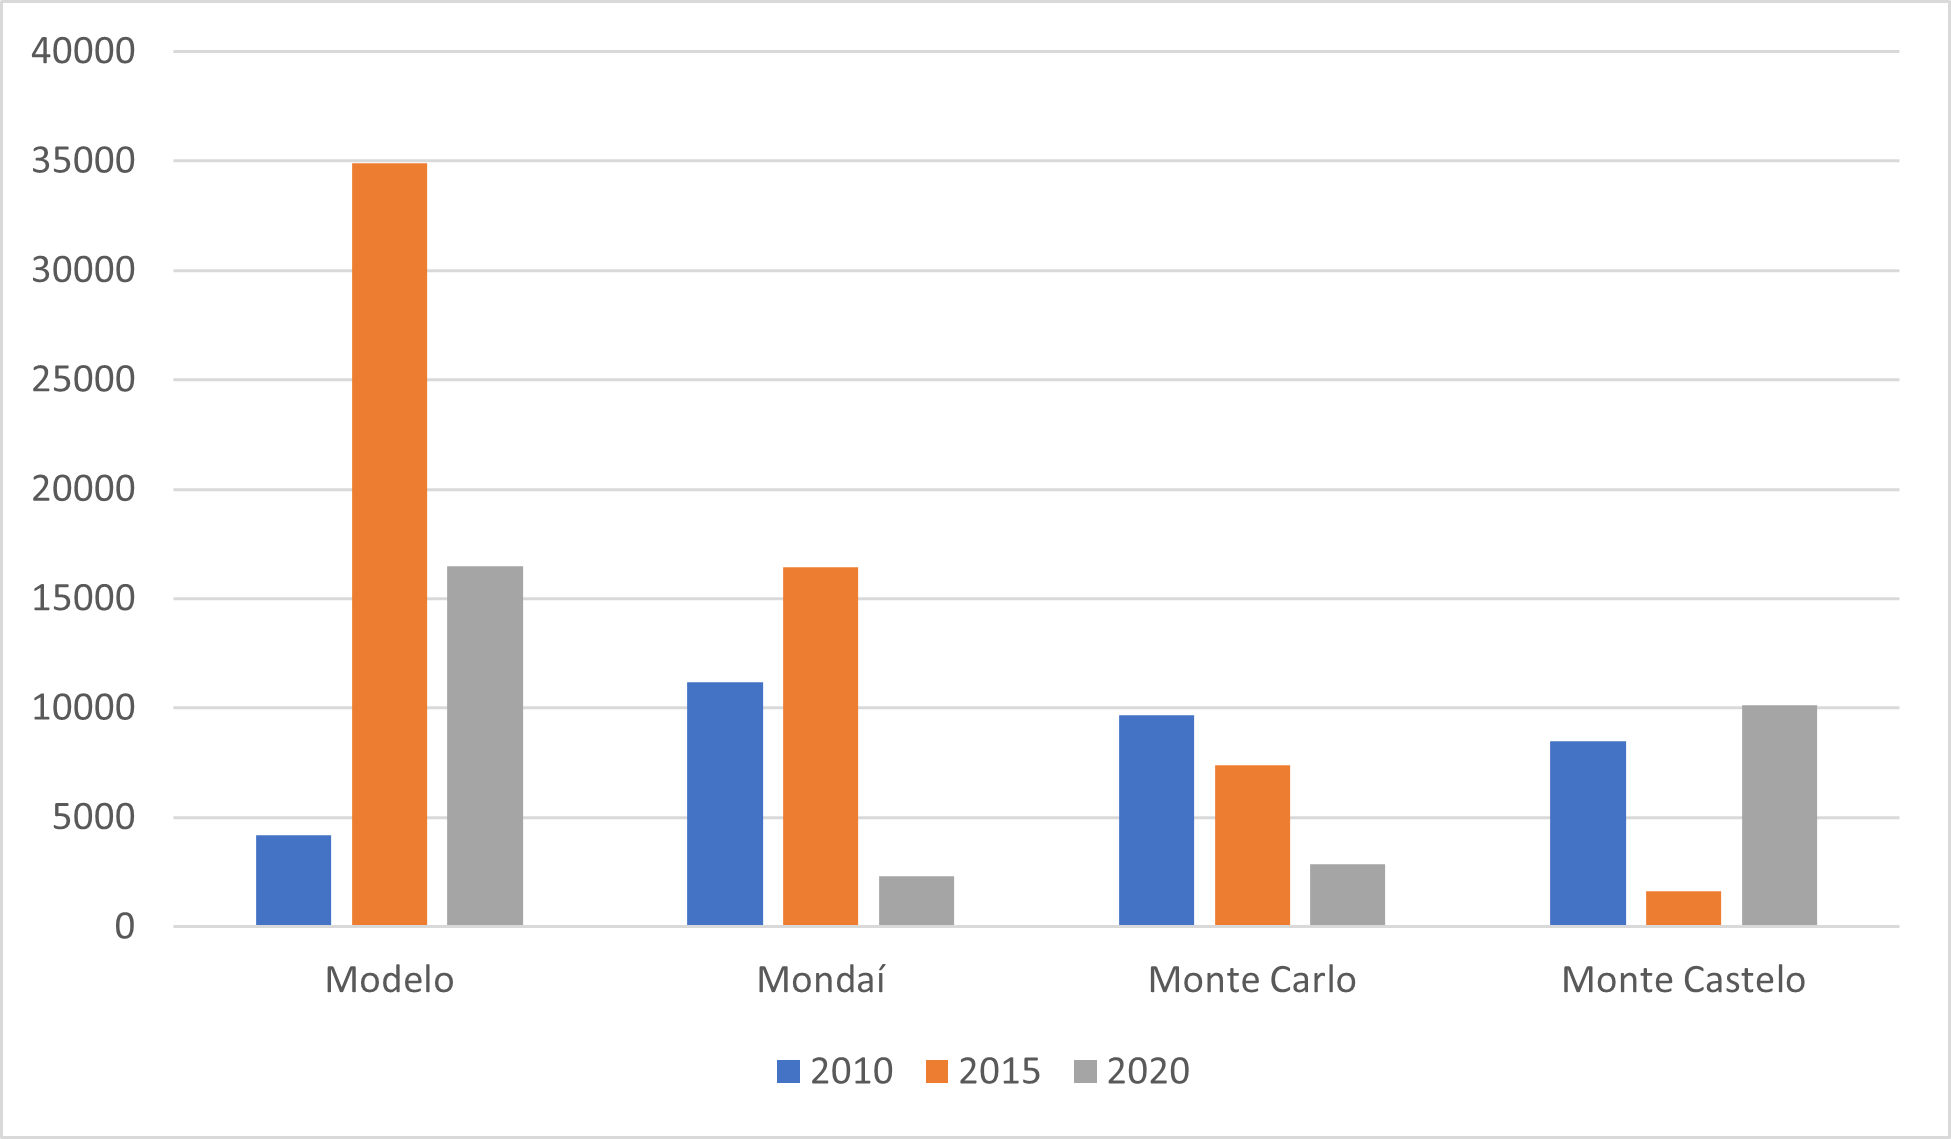
\includegraphics[scale=1]{Textuais/Picture2.png}
	\fonte{\me{2020}}
\end{figure}

As chamadas às equações e fórmulas, no texto, devem ser feitas da seguinte forma: equação (1), fórmula (2).

\textbf{Exemplo 1:}
O Teorema de Pitágoras, é uma equação \eqref{eq:eq1} que pode ser aplicada em qualquer triângulo retângulo (triângulo que tem um ângulo de 90°).
\begin{equation} \label{eq:eq1}
a^2 + b^2 = c^2 
\end{equation}

\textbf{Exemplo 2:}
A dopamina é um composto orgânico de função mista álcool, fenol e amina que apresenta fórmula \eqref{eq:form1} molecular:
\begin{equation} \label{eq:form1}
\ch{C8 + H11NO2} 
\end{equation}

\textbf{Exemplo 3:}
O modelo matemático de Huang (HUG), dado pelas equações \eqref{eq:eq3} e \eqref{eq:eq4}, foi elaborado com o intuito de fornecer uma descrição mais simples do crescimento bacteriano.
\begin{gather} 
	y(t) = y_0 + y_{max} -\ln{[e^{y_0}  + (e^{y_{max}} -e^{y_0} )  e^{-u_{max}\beta(t)} ]}   \label{eq:eq3}  \\
	\beta(t) = t + \frac{1}{4}\ln\left( \frac{1+ e^{-4(t-\lambda)} }{1+ e^{4(\lambda)} }\right) \label{eq:eq4}
\end{gather}
\noindent onde $y(t)$ corresponde ao logaritmo natural da concentração celular (log UFC/g) no instante $t$ (dias), $y_{max}$ é o logaritmo natural da população bacteriana (log UFC/g) final, $y_0$ corresponde ao logaritmo natural da população bacteriana inicial (log UFC/g) e $\beta(t)$ é a função de transição.

\textbf{Exemplo 4:}
Para o cálculo da intensidade fórmula \eqref{eq:eq5} de Intensidade-Duração-Frequência apresentada, os valores encontrados seguindo os parâmetros apresentados e como o resultado é dado em mm/h haverá também a sua conversão para m/s.
\begin{gather} 
	i = \frac{K T^m}{(t+b)^n}   \label{eq:eq5}  \\[2ex]
		i = \frac{\num{625.58} \cdot 5^{\num{0.171}}  }{(60+\num{8.89})^{\num{0.961}}} \\[2ex]
		i = \num{44.222} \cdot \frac{\si{mm}}{\si{h}} \cdot \frac{1\mathrm{m}}{\SI{1000}{mm}} \cdot \frac{\SI{1}{h}}{\SI{3600}{s}} 	
\end{gather}
\noindent onde, $i$ é a intensidade média máxima de precipitação, em mm/h; $T$ é o Período de retorno, em anos; $t$ é a duração da chuva, em minutos; $k,m,b,n$ são os parâmetros da equação determinados para cada local.


As citações diretas com até três linhas ``[...] devem estar contidas entre aspas duplas. As aspas simples são utilizadas para indicar citação no interior da citação.'' (ABNT, 2002, p. 2). Devem apresentar autor, ano e página. Quando a indicação de autor estiver dentro de parênteses, o sobrenome deve ser em letra maiúscula. 


As citações diretas com mais três linhas ``[...] devem ser destacadas com recuo de 4 cm da margem esquerda, com letra menor que a do texto utilizado e sem as aspas.'' (ABNT, 2002, p. 2). Ou seja, utilizar fonte tamanho 10 para as citações diretas longas, com espaçamentos simples entre linhas. As citações devem ser precedidas e antecedidas por um (1) espaço de 1,5 entrelinhas. 

\begin{citacao}
Texto texto texto texto texto texto texto texto texto texto texto texto texto texto texto texto texto texto texto texto texto texto texto texto texto texto texto texto texto texto texto texto texto texto texto texto texto texto texto texto texto texto texto texto texto texto. (SILVA, 2020, p. 21).
\end{citacao}


Nas citações indiretas não há necessidade de usar aspas e indicar a página, considerando que é uma paráfrase. Faz-se necessário apresentar o autor e ano.






\noindent Exemplo referência de livro: \cite{exemplo_livro}

\noindent Exemplo referência de livro em meio eletrônico: \cite{exemplo_livroe}

\noindent Exemplo referência de trabalho acadêmico (Dissertação de Mestrado): \cite{exemplo_dissertacao}

\noindent Exemplo referência de trabalho acadêmico (Tese de Doutorado): \cite{exemplo_tese}

\noindent Exemplo referência de artigo: \cite{exemplo_artigo}


\textbf{Para outras referências ver Manual Udesc}: \url{https://www.udesc.br/bu/manuais}









%


\chapter{Desenvolvimento}







%

\chapter{Conclusão}





% -----------------------------------------------------------------
% ELEMENTOS PÓS-TEXTUAIS
% -----------------------------------------------------------------
\postextual

% Você pode comentar os elementos que não deseja em seu trabalho;

% Referências bibliográficas
\bibliography{abntex2-ref_UDESC_2020}	% Elemento Obrigatório

% ----------------------------------------------------------
% Glossário
% ----------------------------------------------------------

%Consulte o manual da classe abntex2 para orientações sobre o glossário.

%\glossary




% ----------------------------------------------------------
% Glossário (Formatado Manualmente)
% ----------------------------------------------------------

\chapter*{GLOSSÁRIO}
\addcontentsline{toc}{chapter}{GLOSSÁRIO}

{ \setlength{\parindent}{0pt} % ambiente sem indentação

\textbf{Ardósia}: Rocha metamórfica sílico-argilosa formada pela transformação da argila sob pressão e temperatura, endurecida em finas lamelas.

\textbf{Arenito}: rocha sedimentária de origem detrítica formada de grãos agregados por um cimento natural silicoso, calcário ou ferruginoso que comunica ao conjunto em geral qualidades de dureza e compactação.

\textbf{Feldspato}: grupo de silicatos de sódio, potássio, cálcio ou outros elementos que compreende dois subgrupos, os feldspatos alcalinos e os plagioclásios.






} % fim ambiente sem indentação


				% Elemento Opcional

% ----------------------------------------------------------
% Apêndices
% ----------------------------------------------------------

% ---
% Inicia os apêndices
% ---
\begin{apendicesenv}

% Imprime uma página indicando o início dos apêndices
%\partapendices

% ----------------------------------------------------------
\chapter{Países da amostra.}
% ----------------------------------------------------------
\begin{table}[H]
    \caption{Países na amostra}
    \label{tab:sample_countries}
    \small % Ajusta o tamanho da fonte para 10 pontos (que é considerado "small" em LaTeX)
    \begin{tabularx}{\textwidth}{l*{3}{>{\raggedright\arraybackslash}X}}
        \toprule
        \textbf{Country} & \textbf{Country} & \textbf{Country} \\
        \midrule
        Albania & Dominican Republic & Lebanon \\
        Algeria & Ecuador & Lesotho \\
        Angola & Egypt & Liberia \\
        Argentina & El Salvador & Libya \\
        Armenia & Estonia & Lithuania \\
        Australia & Ethiopia & Luxembourg \\
        Austria & Fiji & Macedonia \\
        Azerbaijan & Finland & Madagascar \\
        Bahrain & France & Malawi \\
        Bangladesh & Gabon & Malaysia \\
        Belgium & Gambia & Mali \\
        Benin & Georgia & Mauritania \\
        Bhutan & Germany & Mauritius \\
        Bolivia & Ghana & Mexico \\
        Bosnia and Herzegovina & Greece & Moldova \\
        Botswana & Guatemala & Mongolia \\
        Brazil & Guinea & Morocco \\
        Bulgaria & Guinea-Bissau & Mozambique \\
        Burkina Faso & Guyana & Myanmar \\
        Burundi & Haiti & Namibia \\
        Cambodia & Honduras & Nepal \\
        Cameroon & Hungary & Netherlands \\
        Canada & India & New Zealand \\
        Cape Verde & Indonesia & Nicaragua \\
        Central African Republic & Iran & Niger \\
        Chad & Ireland & Nigeria \\
        Chile & Israel & Norway \\
        China & Italy & Oman \\
        Colombia & Jamaica & Pakistan \\
        Congo, Democratic Republic & Japan & Panama \\
        Congo, Republic & Jordan & Papua New Guinea \\
        Costa Rica & Kazakhstan & Paraguay \\
        Cote d'Ivoire & Kenya & Peru \\
        Croatia & Kuwait & Philippines \\
        Cyprus & Kyrgyz Republic & Poland \\
        Czech Republic & Laos & Portugal \\
        Denmark & Latvia & Qatar \\
        Romania & Russia & Rwanda \\
        Saudi Arabia & Senegal & Sierra Leone \\
        Singapore & Slovak Republic & Slovenia \\
        South Africa & Spain & Sri Lanka \\
        Suriname & Swaziland & Sweden \\
        Switzerland & Syria & Tajikistan \\
        Tanzania & Thailand & Togo \\
        Trinidad and Tobago & Tunisia & UAE \\
        Uganda & Ukraine & United Kingdom \\
        United States & Uruguay & Vietnam \\
        Yemen, Republic & Zambia & Zimbabwe \\
        \bottomrule
    \end{tabularx}
\end{table}

\end{apendicesenv}
% ---				% Elemento Opcional

% ----------------------------------------------------------
% Anexos
% ----------------------------------------------------------
%
% ---
% Inicia os anexos
% ---
\begin{anexosenv}

% Imprime uma página indicando o início dos anexos
%\partanexos

% ---
\chapter{TÍTULO}
% ---



\end{anexosenv}
				% Elemento Opcional

%%---------------------------------------------------------------------
%% INDICE REMISSIVO
%%---------------------------------------------------------------------

%\phantompart
%\printindex

%---------------------------------------------------------------------

%%---------------------------------------------------------------------
%% INDICE REMISSIVO (Formatado Manualmente)
%%---------------------------------------------------------------------

\chapter*{ÍNDICE}
\addcontentsline{toc}{chapter}{ÍNDICE}

{ \setlength{\parindent}{0pt}  % ambiente sem indentação
	

Agradecimentos, 6

Análise de robustez em subamostras, 18, 19

Conclusão, 20

Controles adicionais, 16, 17

Dedicação, 4

Descrição dos Dados, 14, 15

Do Artigo Científico de Replicação, 11

Epígrafe, 7

Folha de rosto, 1

Fonte dos Dados, 11

Glossário, 22

Lista de abreviaturas e siglas, 8

Lista de ilustrações, 8

Lista de símbolos, 9

Lista de tabelas, 8

Memória de Regime, 11, 12

Metodologia Empírica, 13

Referências, 21

Resultados, 14

Reprodução das tabelas do artigo original, 15

Reprodução da Tabela 3, 15, 16

Reprodução da Tabela 4, 16, 17

Reprodução da Tabela 5, 17, 18

Reprodução da Tabela 6, 18, 19

Sumário, 10

Título, 1

	
	
	
	
} % fim ambiente sem indentação


		% Elemento Opcional

\end{document}

% -----------------------------------------------------------------
% Fim do Documento
% -----------------------------------------------------------------	